\chapter{Literature Study}\label{Ch2}
This chapter contains a literature study on the most relevant techniques, equipment, and technologies related to this project. Firstly a high-level block diagram of the proposed solution is given where-after the relevant technologies that are commonly available within the scope of the proposed solution are discussed. The different types of temperature transducers, display, and battery technologies related to this project are reviewed and some important methods to measure core body temperature from skin temperatures are discussed. 

\section{High-level block diagram}
In this section a high-level block diagram of the proposed solution is given. The diagram is shown in \autoref{fig:8} and consists of 4 main functional units. 
\begin{figure}[H]
	\centering
	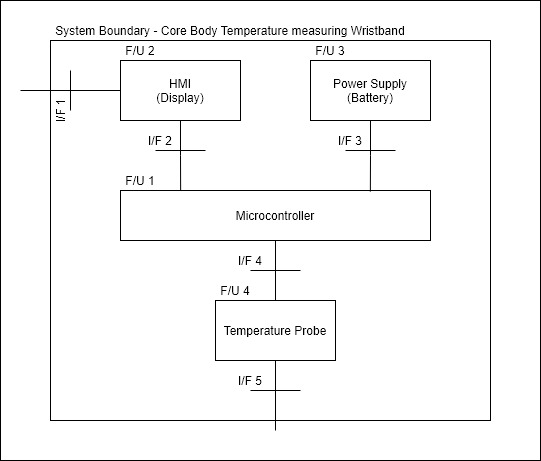
\includegraphics[scale=0.7]{img/High-level-block-diagram}
	\caption{High level block diagram of proposed solution}
	\label{fig:8}
\end{figure}
\noindent
The functional units of the proposed solution are briefly discussed in \autoref{tab:3}.
\begin{table}[H]
	\centering
	\caption{\textit{High-level functional unit description}}
	\label{tab:3}
	\begin{tabular}{|p{8cm}|p{4cm}|}
		\hline
		\textbf{Description} & \textbf{Functional Unit}\\
		\hline
		Analogue to Digital conversion, Processing and analysis of measurements, estimation of core body temperature. & Microcontroller\\
		\hline
		Display the measured temperature. & HMI\\
		\hline
		Deliver power to the system. & Power Supply\\
		\hline
		Measure skin temperature, configuration will allow the microcontroller to estimate core body temperature. & Temperature Probe\\
		\hline
	\end{tabular}
\end{table}

\section{Classification of Body Temperature}
Body temperature measuring dates back to ancient times when physicians used their hands to estimate body temperature by noting the difference in temperature between the head and foot of a patient. As society modernised, more information and technology became available, leading to instruments that can predict and measure body temperature. In practice, the measurement of body temperature is categorised in three distinct types referred to as core body temperature, surface body temperature, and basal body temperature \cite{Chen2019}. The type is determined by considering measurement position. Core body temperature refers to the deep tissue of the body and is the operating temperature of all inner organs. Core body temperature is measured using invasive methods. Surface body temperature is measured on the skin and can be used to estimate core body temperature. Basal body temperature is the lowest body temperature taken right after waking up and before any physical activity and is mostly used to determine and predict ovulation in women \cite{Basal}. There are different places available to measure the body temperature of a human such as sublingual, esophagus, bladder, rectum, and digestive tract for the measurement of core body temperature, and axilla, groin, neck, and wrist for surface body temperature. \\\\
Surface body temperature can easily be measured non-invasively, but can also be susceptible to environmental factors. Since there is a need for a non-invasive body temperature device, the rest of the literature study will focus on surface body temperature measuring techniques, sensing elements, and how to predict core body temperature from surface body temperature. 

\section{Temperature sensing elements}
Temperature sensing elements, or from now on referred to as transducers, convert heat energy or temperature into other forms of energy \cite{Chen2019}. The other forms of energy can then be processed and the temperature can be made visible on a legible temperature scale. This section discusses several temperature transducers that can be used to measure core body temperature. 

\subsection{Thermistor}
Thermistors are semiconductor-resistive temperature transducers where the resistance of the material changes as the temperature changes \cite{Gums2018}. There are two types of thermistors available, the Negative Temperature Coefficient (NTC) thermistor and the Positive Temperature Coefficient (PTC) thermistor \cite{Borwankar2015}. The resistance of an NTC thermistor decreases as the temperature increases and consequently the resistance of a PTC transducer increases as the temperature increases. NTC thermistors are commonly used in body temperature measurements since it has good linearity in the range of body temperature, whereas the PTC thermistor has poor sensitivity in the range of body temperature and are mostly used for higher temperature measurements \cite{Chen2019}. The conversion from resistance to temperature is usually given in the datasheet of the specific thermistor. 

\subsection{Thermocouple}
Thermocouples have two different metal wires connected together as a junction and when the temperature of the junction is changed, the junction output voltage varies with this change \cite{Nookhao2020}. Therefore, the Seebeck effect is used as a thermoelectric transducer \cite{Chen2019}. The Seebeck effect is the phenomenon in which a temperature difference of two dissimilar conductors connected together produces a voltage gradient. This voltage can then be measured and converted to temperature. Several types of thermocouples are available and are classified according to the conductor alloy used inside the thermocouple \cite{Gums2018}. The different types are differentiated by designated letters. Some of the most commonly used thermocouples are shown in \autoref{tab:2}.
\begin{table}[H]
	\centering
	\caption{\textit{Thermocouple types \cite{Maxim2017}}}
	\label{tab:2}
	\begin{tabular}{|c|c|c|}
		\hline
		\textbf{Designated letter} & \textbf{Conductor Alloys (+/-)} & \textbf{Sensing Range (°C)}\\
		\hline
		E & Nickel Chromium / Constantan & -40 to 900\\
		\hline
		J & Iron / Constantan & -180 to 800\\
		\hline
		K & Nickel Chromium / Nickel Aluminium & -180 to 1300\\
		\hline
		N & Nicrosil / Nisil & -270 to 1300\\
		\hline
		T & Copper / Constantan & -250 to 400\\
		\hline
		R/S & Copper / Copper Nickel Compensating & -50 to 1750\\
		\hline
		B & Platinum Rhodium & 0 to 1820\\
		\hline
	\end{tabular}
\end{table}
\noindent
Most applications that use a thermocouple as a temperature transducer, require precise amplification since the output voltage is quite small. This adds circuitry to the measurement device and is not ideal for smaller-sized projects.

\subsection{Resistive Temperature Detector}
Resistive Temperature Detectors or RTDs work on the same principle as thermistors, where the varied resistance of the metal is measured when there is a temperature change. The most common and accurate material used to make RTDs is platinum \cite{Gums2018}. The reason for this is that platinum RTDs offer a nearly linear response to temperature changes, repeatable responses, a wide temperature range, and they are accurate and stable. RTD configurations can be two-/three-/four-wire and is shown in \autoref{fig:2}. An excitation current flows through the RTD and the voltage across the RTD is measured.
\begin{figure}[H]
	\centering
	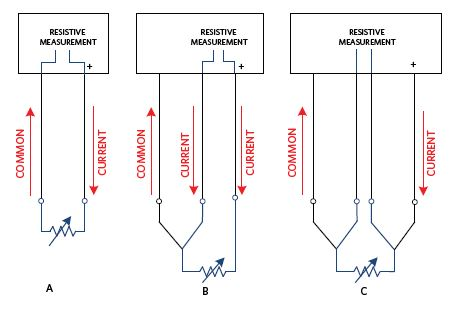
\includegraphics[scale=0.7]{img/RTD-configurations}
	\caption{RTD configurations \cite{Maxim2017}}
	\label{fig:2}
\end{figure} 
\noindent
RTD thermal transducers respond slower than thermocouples to changes in temperature \cite{Gums2018}.

\subsection{Semiconductor based Integrated Circuit}
The semiconductor sensor in an integrated circuit (IC) contains many types of circuitry on one chip \cite{Nookhao2020}. Semiconductor-based IC measures temperature by using the physical properties of a transistor \cite{Gums2018}. The collector current and base-emitter voltage of a bipolar junction transistor (BJT) is used to calculate the measured temperature. The PN junction is therefore used as a temperature transducer. The forward voltage drop across a forward-conducting PN junction of a transistor at constant forward-bias current exhibits linear temperature dependence over a wide temperature range \cite{Chen2019}. Temperature transducers based on this principle can be realised by applying a square-wave current to a PN junction \cite{Verster1968} or by using two matched devices operating at different currents. 

\subsection{Infrared}
The temperature of an object can be measured by the thermal radiation power emitted from the object if the object has a temperature above absolute zero (0 Kelvin). The infrared energy emitted from an object is proportional to its temperature. This method can be used to measure body temperature since the peak of the thermal radiation emitted from a human body lies in the far-infrared region \cite{Chen2019}. The infrared type temperature transducer can make temperature measurements contactless. Most infrared temperature transducers use a pyroelectric sensor to measure temperature. 


\section{Techniques for Non-invasive CBT measurements}\label{Sec2_4}
Several non-invasive methods have been developed to measure core body temperature since the early 1970s \cite{Chen2019}. The reason for this is that some core body temperature measuring techniques are unsatisfactory for continuous use and may cause discomfort to the patient \cite{Yamakage2003}. Furthermore, some invasive measurements can induce complications \cite{complications}. The working of the developed methods is discussed next. 

\subsection{Zero-heat-flow Method}
The zero-heat-flow method is used to estimate core body temperature in a non-invasive manner. The estimation is made by measuring the temperature on the skin surface with a probe that consists of two thermistors, a thin-film heater element, and a piece of nylon used as a thermal insulator. These components are encapsulated by silicone rubber and the structure can be seen in \autoref{fig:3}.
\begin{figure}[H]
	\centering
	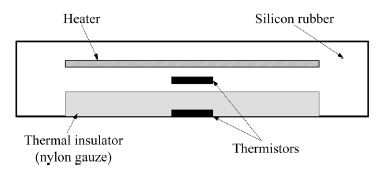
\includegraphics[scale=0.8]{img/zero-heat-flow}
	\caption{Zero-heat-flow structure\cite{Chen2019}}
	\label{fig:3}
\end{figure} 
\noindent
The heater element is used to reduce ambient effects on measurements \cite{Matsunaga2020}. The method is based on heat or thermal insulation to reduce heat loss from the skin. Two matched thermistors are used to detect the temperature on both sides of the insulating layer and these temperatures are then compared. The temperature difference between them is used to control the heater current in such a way that there is no temperature gradient across the insulating layer, therefore no heat flowing through this layer \cite{Yamakage2003}. As long as the condition of zero-heat-flow is satisfied, the probe can be seen as an ideal thermal insulator, and heat loss from the skin is prevented. After a while (around 15 minutes), the skin temperature will be in equilibrium with deep tissue temperature and the lower thermistor that is in contact with the skin may be used to measure skin temperature \cite{Yamakage2003}.
\\
\\
Since a heater element is present in this method, it requires a substantial amount of power. This, together with the relatively big size is not ideal for low-energy, smaller-sized projects.

\subsection{Dual-heat-flux Method}
In response to the zero-heat-flow method mentioned above that needs a heater element, the dual-heat-flux method was developed that works without a heating element \cite{Kitamura2010}. The measurement probe is built structurally to form two different thermal pathways, hence the name dual-heat-flux. Temperature is measured by temperature transducers at the end of each channel. The structural layout of this method is shown in \autoref{fig:4}.
\begin{figure}[H]
	\centering
	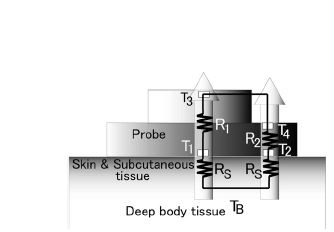
\includegraphics[scale=0.9]{img/dual-heat-flux}
	\caption{Dual-heat-flux structure\cite{Kitamura2010}}
	\label{fig:4}
\end{figure} 
\noindent
From the schematic diagram above, the two channels of heat flow and the equivalent circuit can be seen. The skin is covered by two kinds of heat insulators that have different thermal resistances, $R_{1}$ and $R_{2}$, $R_{s}$ is the thermal resistance of the subcutaneous tissues and skin, $T_{1}$ and $T_{2}$ are the skin temperatures under the insulator, and $T_{3}$ and $T_{4}$ are the upper temperatures at the surface of the insulator \cite{Chen2019}. $T_{B}$ is the core body temperature that needs to be measured. Kitamura et al. \cite{Kitamura2010} derived the following equation to estimate core body temperature by assuming that $R_{s}$ of both channels are identical:
\begin{equation}
	T_{B} = T_{1} + \frac{(T_{1} - T_{2})(T_{1} - T_{3})}{K(T_{2} - T_{4})(T_{2} - T_{4})}
	\label{1}
\end{equation}
\noindent
$K$ is the ratio of thermal resistance and can be determined from \autoref{1} by rearranging the terms and conducting experimental calibration in a water bath:
\begin{equation}
	K = \frac{(T_{B} - T_{2})(T_{1} - T_{3})}{(T_{B} - T_{1})(T_{2} - T_{4})}
\end{equation}
where, $T_{B}$ can be set to the preset water temperature. 
\\
\\
This method has shown promising results, however, underlying skin anatomy and ergonomics still remain an issue \cite{Atallah2018}. In this method $R_{s}$ of both channels are presumed to be identical since two insulators are placed close to each other, resulting in $K$ not being influenced by $R_{s}$. However, Feng et al. \cite{Feng2017} found that $K$ is a function of the thickness of the skin or body, and $R_{s}$ cannot be cancelled out once $R_{s}$ changes. $R_{s}$ will change with different skin types, colours, and thicknesses. Feng et al. \cite{Feng2017} also revealed that the dual-heat-flux method has a long measurement time and systems based on this method are relatively large.

\subsection{Thermal equivalent circuit model}
The dual-heat-flux method does not take ambient conditions into consideration and heat flux from core body temperature may uncontrollably leak directly into the ambient environment instead of being measured by the transducers mentioned in the dual-heat-flux method \cite{Matsunaga2020}. Another method to measure core body temperature from the skin surface is to use the thermal equivalent circuit model to estimate core body temperature with a skin-attachable probe. 
\\
\\
The thermal equivalent circuit for a skin-attachable sensor for the core body temperature estimation model was first developed by Fox et al. \cite{Fox1973}. An amended thermal equivalent circuit can be seen in \autoref{fig:1} of this report. The core body temperature ($T_{core}$) is estimated by the following:
\begin{equation}
	T_{core} = T_{skin} + (R_{body} \times H_{skin})
\end{equation}
where the skin surface temperature, the measured heat flux and the thermal resistance of the body are denoted by $T_{skin}$, $H_{skin}$ and $R_{body}$ respectively. Matsunaga et al. \cite{Matsunaga2020} developed an improved thermal equivalent circuit model which takes the uncontrolled heat flux leak to the ambient environment, and external convection changes into consideration. The improved thermal equivalent circuit is shown in \autoref{fig:5}.
\begin{figure}[H]
	\centering
	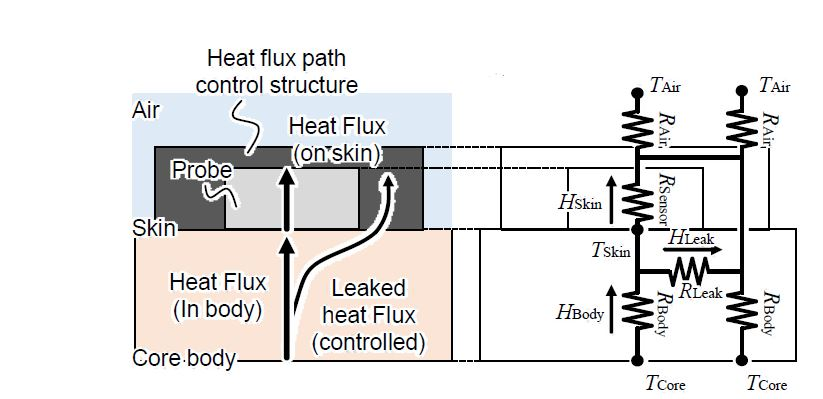
\includegraphics[scale=0.6]{img/improved-temp-model}
	\caption{Improved thermal equivalent model \cite{Matsunaga2020}}
	\label{fig:5}
\end{figure}
\noindent
In this figure, the thermal resistance of the probe, heat flux in the body, the ambient temperature, and thermal resistance to ambient air are denoted by $R_{sensor}$, $H_{body}$, $T_{air}$ and $R_{air}$ respectively. $R_{leak}$ and $H_{leak}$ denote the thermal resistance of the leakage path and the leaked heat flux. Matsunaga et al. \cite{Matsunaga2020} then gives the core body temperature ($T_{core}$) as the following:
\begin{equation}
	T_{core} = T_{skin} + (R_{body} \times \alpha H_{skin})
\end{equation}
\noindent
$\alpha$ is the calibration coefficient and is given by:
\begin{equation}
	\alpha = \frac{(H_{skin} + H_{leak})}{H_{skin}}
\end{equation}
\noindent
By using $H_{skin}$ and $H_{leak}$ together with Kirchhoff's first and second laws, $\alpha$ can be rewritten as a function of thermal resistance:
\begin{equation}
	\alpha = 1 + \frac{R_{sensor}}{R_{leak}}
	\label{6}
\end{equation}
\noindent
From \autoref{6} it is clear that $\alpha$ does not depend on $R_{air}$ which means that the calibration coefficient does not change by changes in ambient conditions, and consequently, estimation errors do not occur. Through this process, Matsunaga et al. \cite{Matsunaga2020} considered $R_{body}$ and $R_{leak}$ as constant since they mainly depend on the thickness of the human body at the point of measuring. $R_{sensor}$ is also constant. To control the heat flux path, the probe is wrapped with a highly conductive material to ensure that the leaked heat flux is passing through the thermally conductive material. 
\\
\\
It is clear that the thermal resistance of the body is still needed to use this method. When using an average value for $R_{body}$ estimation errors may occur that impacts the accuracy of the method. It is also generally quite difficult to obtain the thermal resistance of the leakage path. 

\subsection{Statistical Estimation}\label{stat}
This method estimates core body temperature from skin temperatures by following a  technique that is completely different from the previous methods. Kwak et al. \cite{Kwak2019} proposed a statistical estimation of core body temperature from skin temperature. In this method, the central limit theorem of statistics is used to overcome the problems faced when using a skin-attachable sensor to measure core body temperature. One of the major problems that are faced is that skin temperature is affected by external conditions such as wind and ambient temperature. The central limit theorem states that if there is a population with a mean and a standard distribution and many samples are taken from the population, the distribution of the sample means will be approximately normally distributed \cite{Sang2017}. In other words, arbitrary distributions are normally distributed as the number of samples increases. Kwak et al. \cite{Kwak2019} uses this theorem to obtain a normal distribution of skin temperature and core body temperature and map each normal distribution to each other. 
\\
\\
This method requires a lot of data or samples to increase its accuracy. Therefore, many measurements should be made on the ambient temperature, the skin temperature and the core body temperature. After a generous amount of data is gathered, the statistical model can be build. The following steps are followed to build the statistical model \cite{Kwak2019}:
\begin{enumerate}
	\item Draw boxplot:\\
	A boxplot is a standard way of showing the distribution of data by providing a five number summary(minimum, first quartile, median, third quartile, and maximum). Outliers from the data model based on core body temperature are excluded since some measurements may be erroneous. 
	\item Draw histograms:\\
	A histogram of skin temperature and core body temperature should be drawn respectively. The histograms are then used to find the fitting Gaussian functions for skin temperature and core body temperature. The Gaussian functions for skin temperature and core body temperature are respectively:
	\begin{eqnarray}
		skin\_gauss(x) = a_{1} \times \exp [-(\frac{x-a_{2}}{a_{3}})^2]\\
		body\_gauss(y) = b_{1} \times \exp [-(\frac{y-b_{2}}{b_{3}})^2]
	\end{eqnarray}
	where $x$ is a random variable for skin temperature, $y$ a random variable for core body temperature, $a_{1}$, $b_{1}$ the amplitudes, $a_{2}$, $b_{2}$ the centroids and $a_{3}$, $b_{3}$ the peak widths. 
	\item Map the Gaussian function of skin temperature to the Gaussian function of core body temperature:\\
	The Gaussian function of skin temperature is firstly mapped to a standard normal distribution and then the standard normal distribution is mapped to the Gaussian function of core body temperature. A relevant example of the mapping is shown in \autoref{fig:6}.
	\begin{figure}[H]
		\centering
		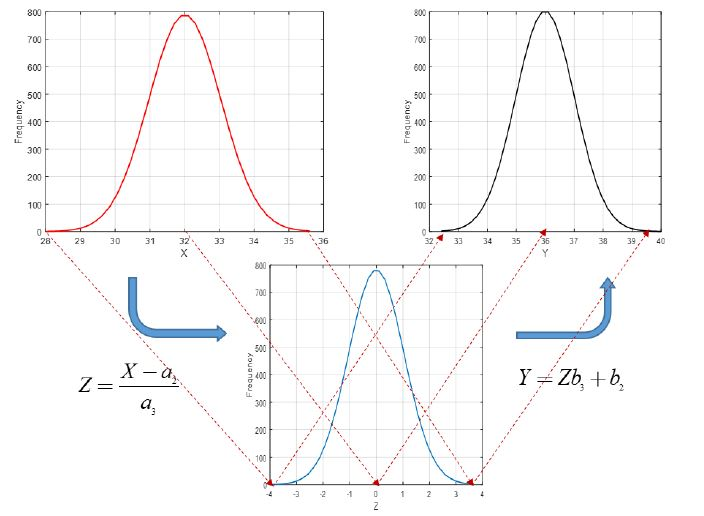
\includegraphics[scale=0.5]{img/stats-mapping}
		\caption{Mapping of Gaussian functions \cite{Kwak2019}}
		\label{fig:6}
	\end{figure}
	\noindent
	where the corresponding formula is given by:
	\begin{equation}
		Y = b_{3}(\frac{X - a_{2}}{a_{3}}) + b_{2}
	\end{equation}
\end{enumerate}
\noindent
Kwak et al. \cite{Kwak2019} concluded that the statistical method estimates core body temperature reliably and that the estimated core body temperatures are within the margin of error tolerance of actual thermometers. The main drawback of this method is that a lot of data or samples are needed to build a statistical model that will deliver reliable results. 


\section{Display Technologies} 
Many display technologies and modules coexist and compete for their share in the market \cite{Fer2015}. The term display in this context is referring to an output device that can exhibit, show or project information to visually communicate with a user. This section will focus on the most widely used display technologies that are available for low power consumption applications.
\\
\\ 
Fernández et al. \cite{Fer2015} reviewed the display technologies available, focusing on the power consumption of each technology. The following figure shows the power consumption density of the various display technologies:
\begin{figure}[H]
	\centering
	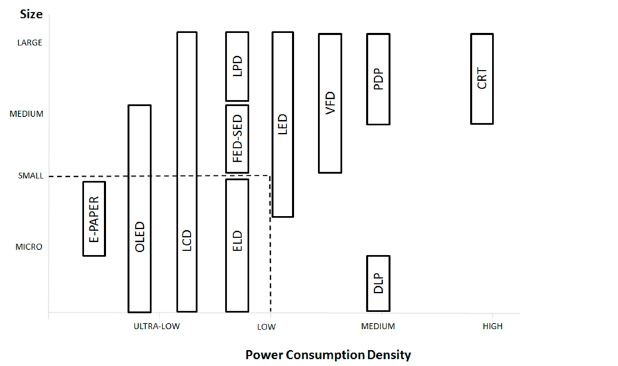
\includegraphics[scale=0.9]{img/Display-power}
	\caption{Power Consumption Density of Display Technologies \cite{Fer2015}}
	\label{fig:7}
\end{figure}
\noindent
From \autoref{fig:7} the technologies that consume low, and ultra-low power can be determined. These display technologies that are commonly used will be briefly discussed next. 

\subsection{E-PAPER}
E-PAPER (Electronic paper)  is a display technology designed to mimic the appearance of ordinary in on paper \cite{Joseph2016}. Millions of microcapsules containing negatively charged black and positively charged white particles suspended in a clear liquid are the composition of the display \cite{Fer2015}. This technology does not require a backlight to illuminate its pixels and is made from a flexible material that requires ultra-low power to operate. E-Paper is also easier to read at an angle compared to flat-screen monitors.

\subsection{LPD}
LPD (Laser Phosphor Display) is a breakthrough phosphor screen technology that is powered by a laser engine. LPD uses solid state lasers to excite phosphors, and as the lasers scan the surface, the phosphors emit red, green, and blue colours that generate high-resolution images \cite{Hajjar2010}. The lasers modulate by turning on and off for each pixel to create an image.

\subsection{LED}
LED (Light-Emitting Diodes) are opto-semiconductors that convert electrical energy into light energy. This technology emits light by applying a voltage to an inorganic semiconductor \cite{Zissis2014}. An electronic display screen has many independent arranged pixels and full colour LED displays select red, green, and blue as primary colours where each pixel consist of an LED \cite{Ni2013}. The colour of the LED is realised by controlling the LED brightness i.e. the current through the semiconductor.

\subsection{OLED}
An OLED (Organic Light-Emitting Display) is an LED in which the emissive electroluminescent layer is an organic compound film, hence, it is a solid-state device made of a thin, carbon-based semiconductor layer that emits light when an electric current is applied \cite{Zissis2014}.

\subsection{LCD}
LCD (Liquid Crystal Display) technology consists of an array of tiny segments that can be manipulated, using polarization of lights, to present information. This display technology belongs to the non-emissive display category, meaning that a backlight is included in the design, which in turn means that slightly more power than OLED and E-PAPER is consumed \cite{Fer2015}.

\subsection{ELD}
ELD (Electroluminescent Display) technology uses a strong electric field to take advantage of the light-emission phenomenon \cite{Fer2015}. ELDs consists of a solid state thin phosphor film and insulator stack deposited on a glass substrate that is driven by a high voltage which generates alternating positive and negative pulses \cite{King}. ELDs do not require a backlight and are therefore energy efficient.

\section{Power supply}
In \autoref{1.7} of this report, it is mentioned that the core body temperature device must be portable and relatively small. This indicates that the device will have an onboard power supply unit in the form of a small battery. First, the difference between a battery and a cell is discussed. The basic difference between a battery and a cell is that a cell is an energy source that delivers DC voltage and current in small quantities, where the functionality of a battery is the same but is arranged in a series or parallel fashion so that voltage levels could be raised \cite{Components2019}. This section shortly describes commonly found batteries in small applications.  

\subsection{Primary Batteries}
These types of batteries are known as non-rechargeable batteries and can only be used once. The commonly non-rechargeable batteries used in smaller applications are:
\begin{itemize}
	\item Alkaline batteries:\\
	The chemical composition of this type of battery is Zinc ($Zn$) and Manganese dioxide ($MNO_{2}$) with an electrolyte of potassium hydroxide \cite{Components2019}. This battery is in a small cylindrical form and the cost is relatively high. 
	\item Button / Coin cell batteries:\\
	Lithium and silver oxide chemicals are used as a chemical composition for a coin or button cell battery, although these are also alkaline in nature \cite{Components2019}, \cite{Battery2019}. Coin cell batteries have a thin, small circular shape and are lightweight with a high nominal voltage ($\pm$3V), but the drawback is that they need a holder. 
\end{itemize}

\subsection{Secondary Batteries}
Secondary batteries are also known as rechargeable batteries that can be reused. Some commonly used rechargeable batteries in small applications are:
\begin{itemize}
	\item Li-ion batteries:\\
	These batteries are made of Lithium metal and are used in portable applications which need high power \cite{Components2019}. Li-ion batteries are very lightweight with a high cell voltage, but a battery protection circuit is needed in the desired application since the battery might explode when the terminals are short-circuited. 
	\item Li-Po batteries:\\
	Li-Po batteries use polymer gel or polymers electrolyte instead of liquid electrolyte and are mostly the same as the Li-ion technology \cite{Components2019}. Compared to Li-ion batteries, these batteries are highly protected and may be more expensive. 
	\item Ni-Cd batteries:\\
	The chemical composition of these batteries is Nickel and Cadmium with a low discharge rate \cite{Components2019}. To avoid the growth of crystals on the battery plate, these batteries must be charged more frequently.
	\item Ni-MH batteries:\\
	These are Nickel – Metal Hydride batteries, and although these batteries have a high self-discharge rate, they are much more preferred than Ni-Cd batteries as they have a lower impact on the environment \cite{Components2019}. 
\end{itemize}

\section{Concluding Remarks}
This section reviewed the most commonly used temperature transducers, display technologies, and battery types used in a smaller type of applications. Several methods were discussed to estimate core body temperature from skin surface temperature more accurately without the measurements getting affected by external factors such as ambient temperatures and wind.

